% Show distributions for loose cuts, 5e19 data/MC comparison
% Aggressive cuts, 6.6e20 Projection
% Current efficiency and purity plots as a function of energy

\section{Electron-Like Event Distributions}\label{sec:electron_like}
\subsection{Reconstructed energy spectrum}
The reconstructed energy spectrum of the selected events after the application of the background-rejection cuts is shown in Figure \ref{fig:spectrum_after}. It corresponds to the sum of the reconstructed energies of the shower-like objects, as described in Section \ref{sec:showerenergy}, and the reconstructed energies of the track-like objects, as described in Section \ref{sec:protonenergy}. 

\begin{figure}[htbp]
\centering
  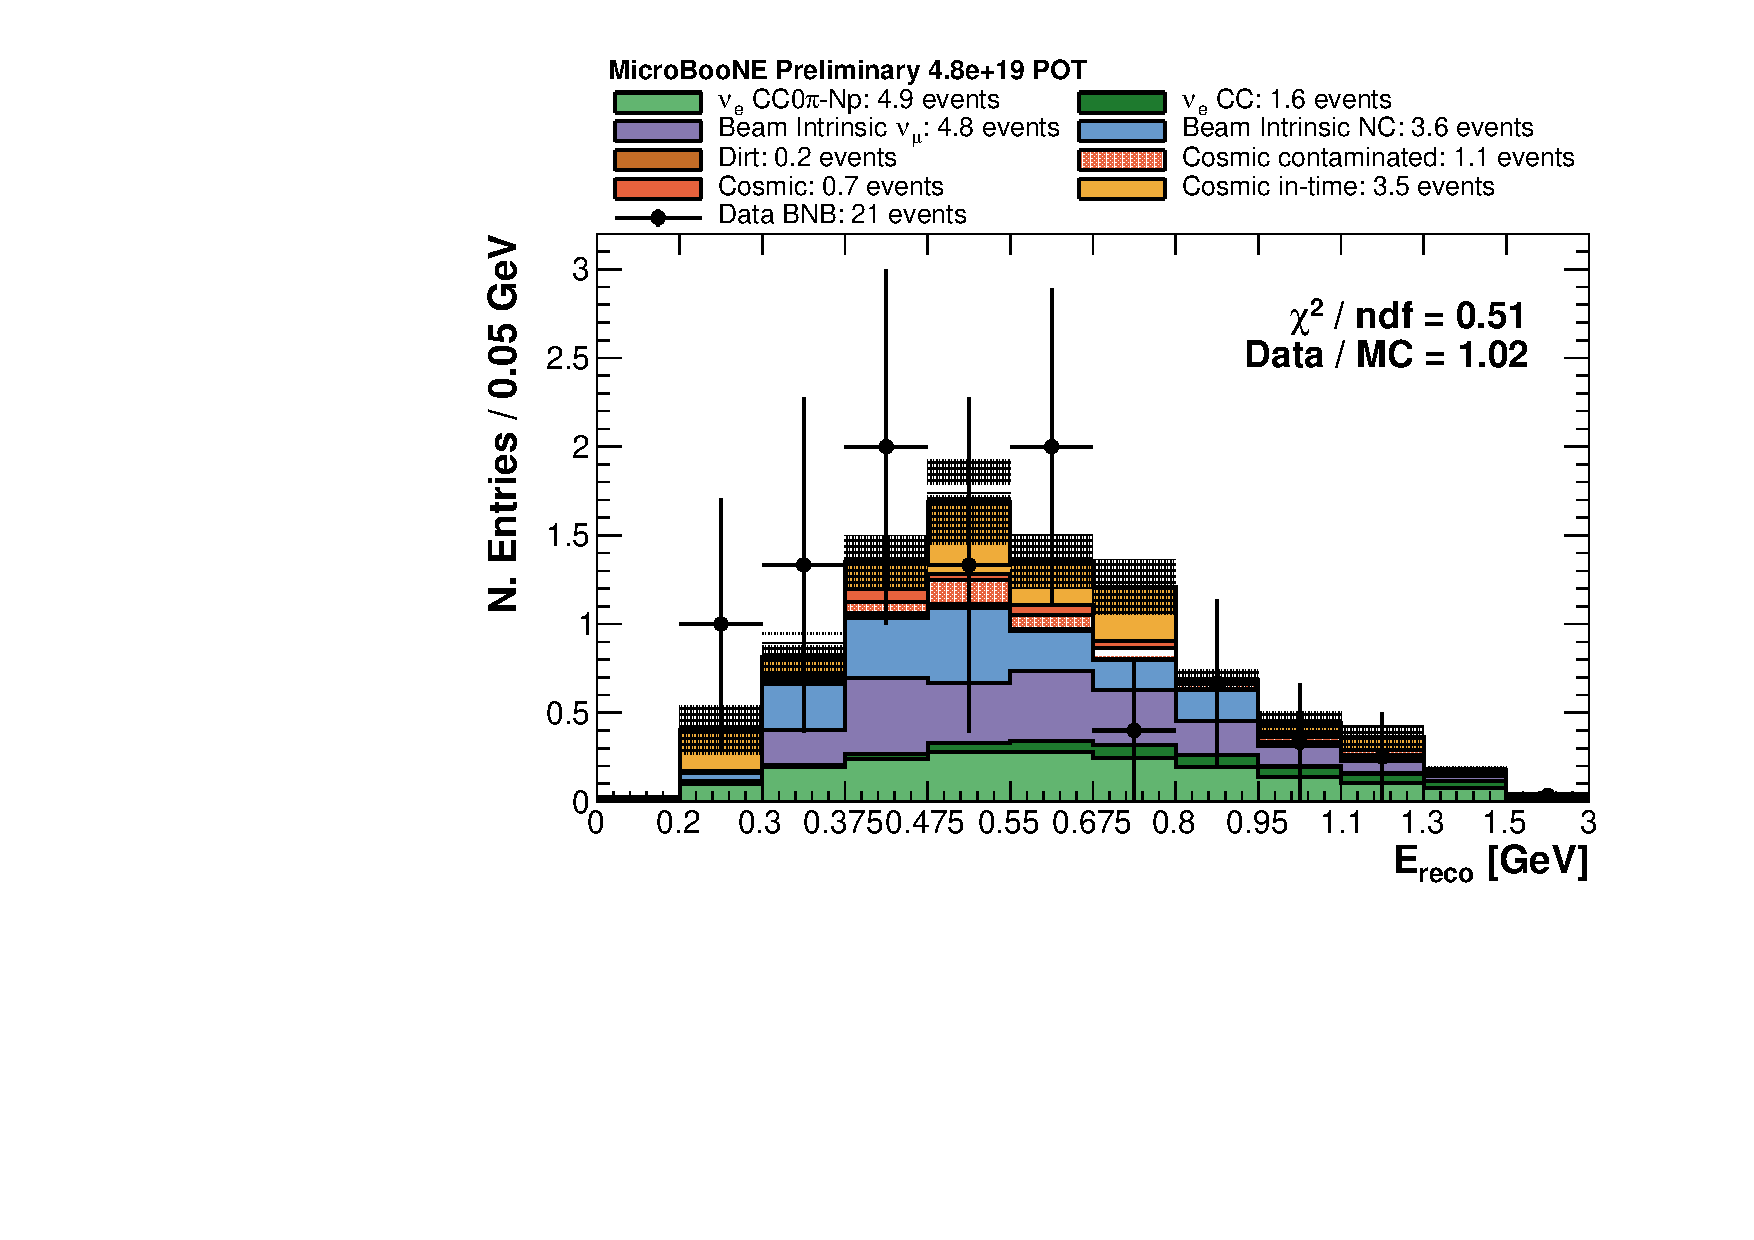
\includegraphics[width=0.65\linewidth]{figures/h_fixed_energy_after.pdf}
    \caption{Reconstructed energy spectrum of the selected events after the background-rejection cuts.}\label{fig:spectrum_after}

\end{figure}

The final number of selected data events in the unblinded data sample is 21, corresponding to a MicroBooNE exposure of \num{4.84e19} POT. These events have been hand-scanned: Figure \ref{fig:evds} shows the event displays of two $\nu_{e}$-like selected data events.

\begin{figure}[htbp]
\centering
  \begin{subfigure}{0.7\textwidth}
  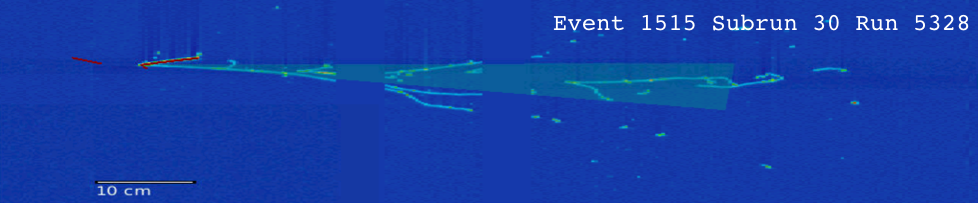
\includegraphics[width=\linewidth]{figures/data1.png}
    \caption{Event 1515, Subrun 30, Run 5328}
\end{subfigure}
  \begin{subfigure}{0.7\textwidth}	
  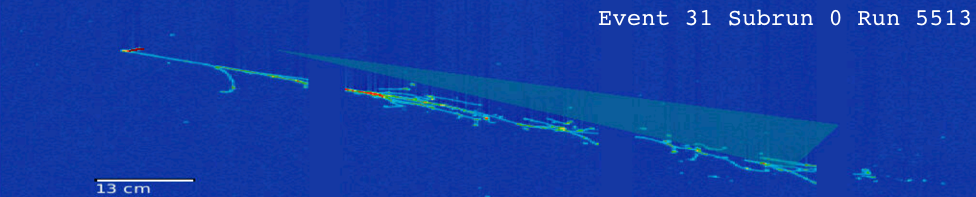
\includegraphics[width=\linewidth]{figures/data2.png}
  \caption{Event 31, Subrun 0, Run 5513}
\end{subfigure}

  \caption{Event displays of the collection plane of two $\nu_{e}$-like data events present in our sample after the background-rejection cuts. The gaps are caused by the presence of missing or unresponsive wires. The red lines correspond to reconstructed track-like objects and the green cones correspond to reconstructed shower-like objects. }
  \label{fig:evds}
\end{figure}

The data BNB distribution is in good agreement with the stacked Monte Carlo + EXT distributions, both in normalization (the integral ratio is 1.02) and in shape ($\chi^2 /\mathrm{n.d.f.} = 0.51$). 

The events selected in the different neutrino components ($\nu_{e}$ CC0$\pi$-Np, $\nu_{e}$ CC, beam intrinsic $\nu_{\mu}$, beam intrinsic NC, and outside fid. vol.) can also be categorized according to the process responsible of the interaction. Figure \ref{fig:interactions} shows the reconstructed energy spectrum for each GENIE interaction type, after the boxed cuts. 

\begin{figure}[htbp]
\centering
  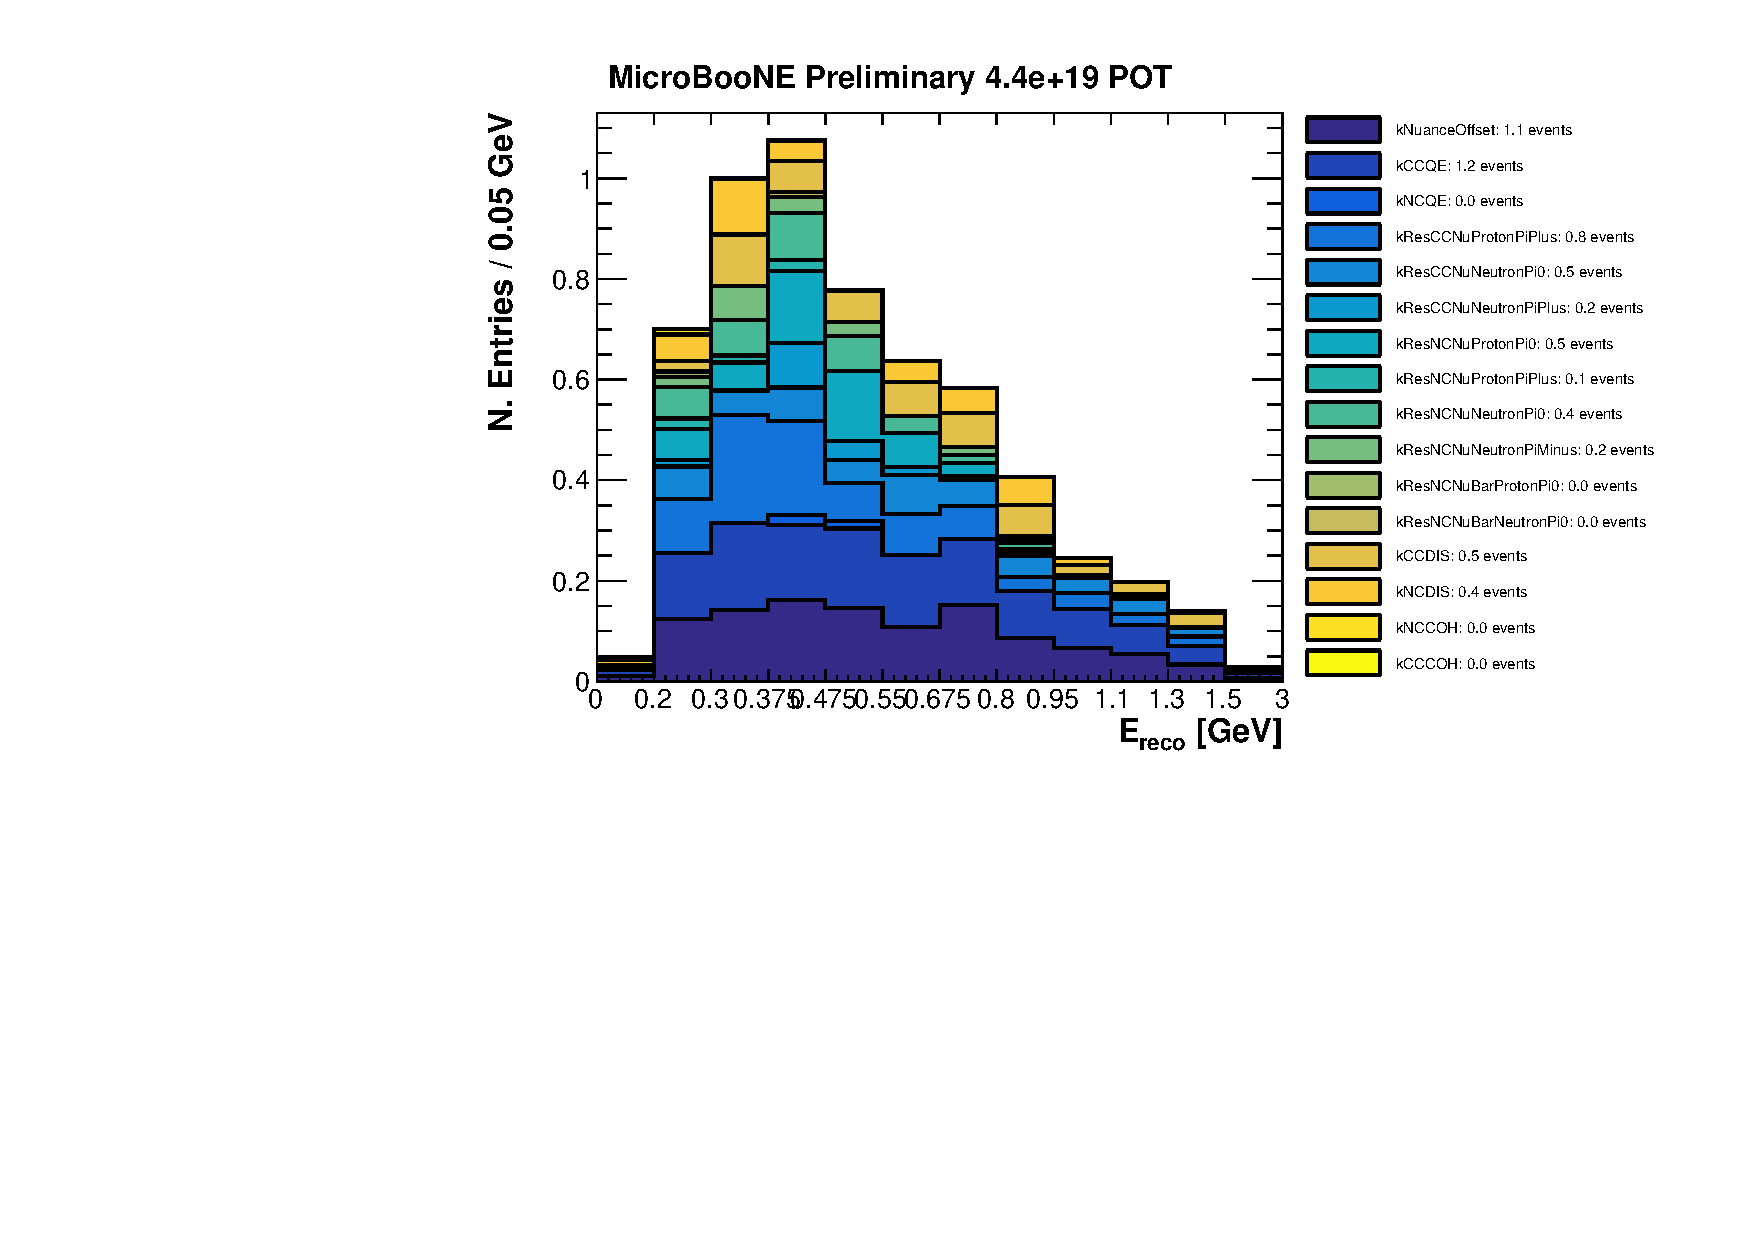
\includegraphics[width=0.65\linewidth]{figures/h_interactions.pdf}
    \caption{Reconstructed energy spectrum of the neutrino components, categorized according to their GENIE interaction name.}\label{fig:interactions}

\end{figure}

\subsection{Angular and spatial distributions}
In this section we study the agreement between the data and Monte Carlo distributions for spatial (in the $x$, $y$, and $z$ coordinates) and angular (inclination $\theta$ and azimuth $\phi$) distributions, after the boxed cuts.
Figure \ref{fig:showerxyz} shows the distributions of the starting point of the most energetic reconstructed shower in each event in the spatial coordinates. The agreement between data and simulation is good, however it is not possible to draw any conclusions on the spatial distributions due to the limited statistics. 

\begin{figure}[htbp]
\centering
  \begin{subfigure}{0.3\textwidth}
    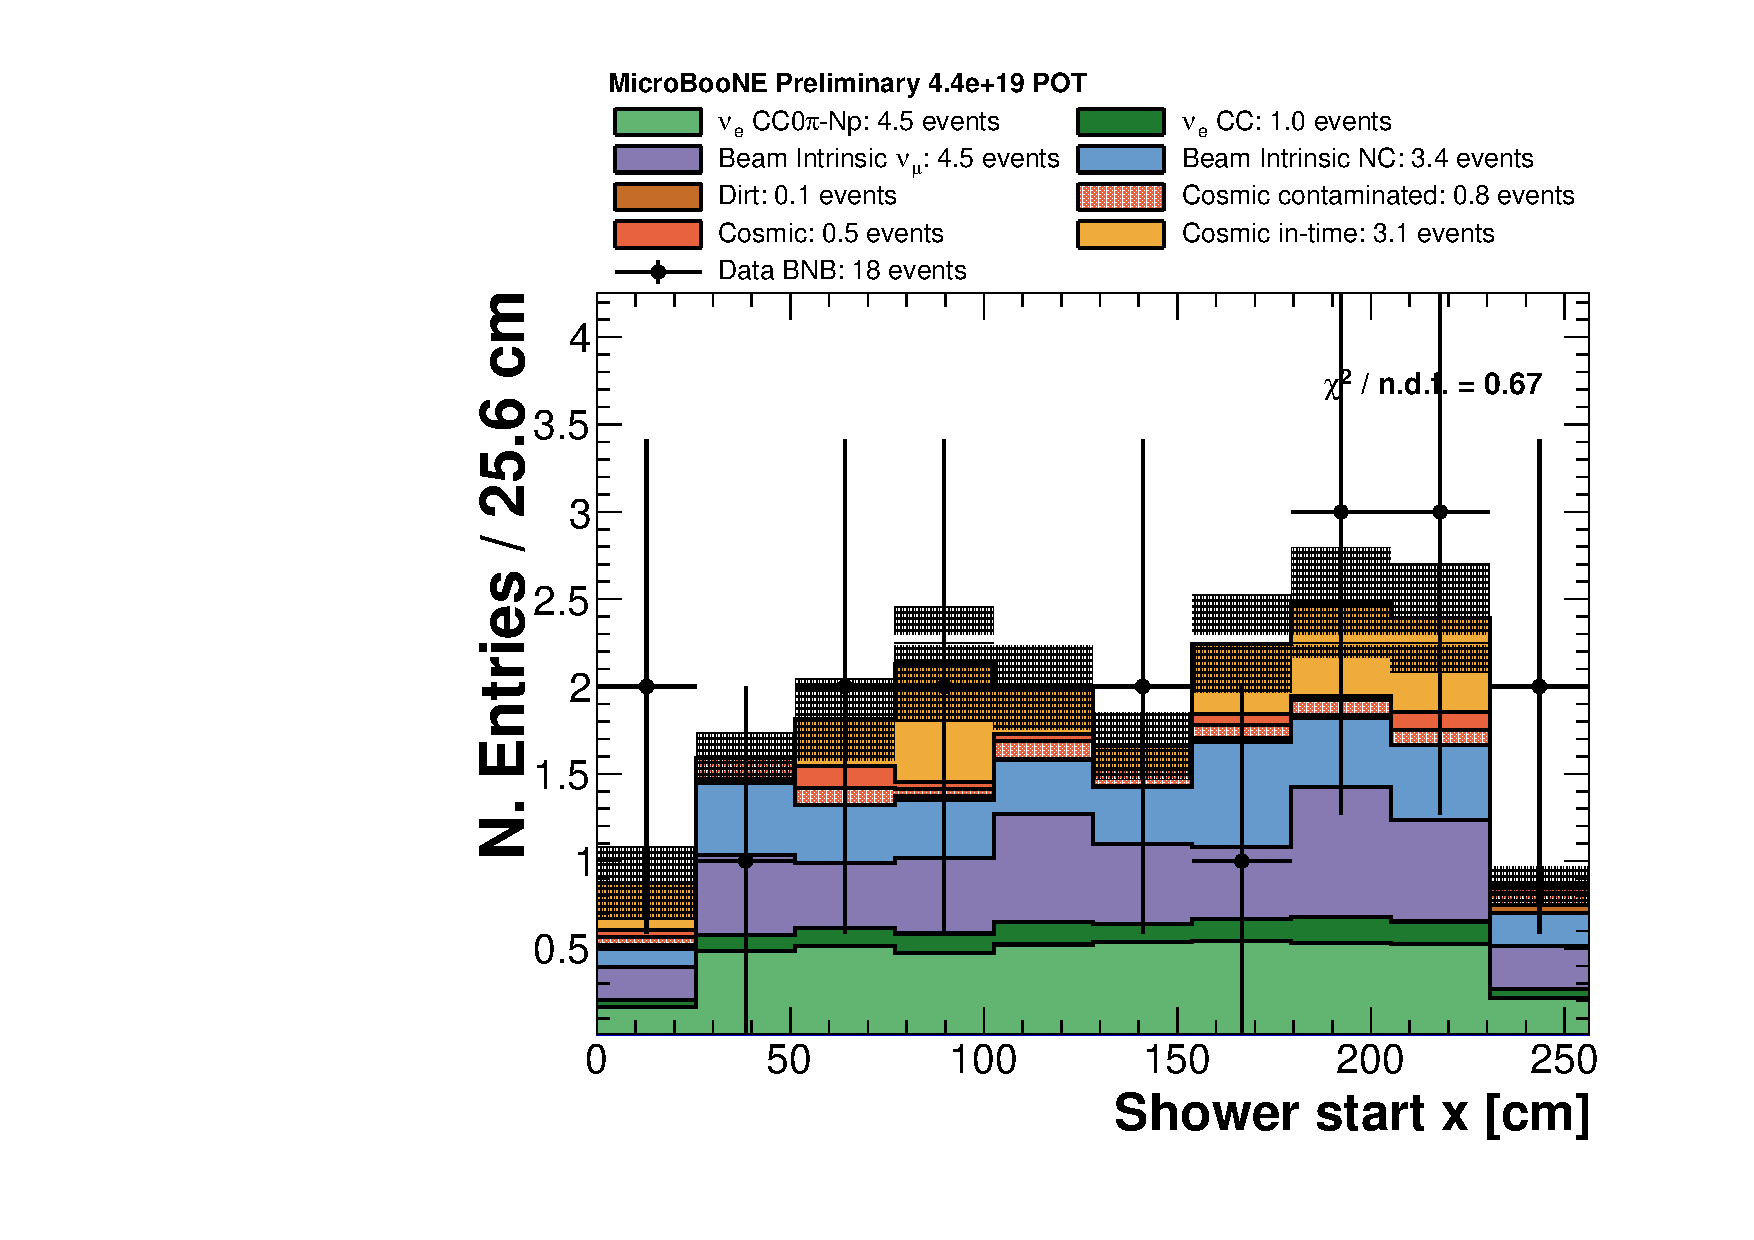
\includegraphics[width=\linewidth]{figures/h_shower_start_x.pdf}
    \caption{$x$ coordinate.} 
  \end{subfigure}
  \begin{subfigure}{0.3\textwidth}
    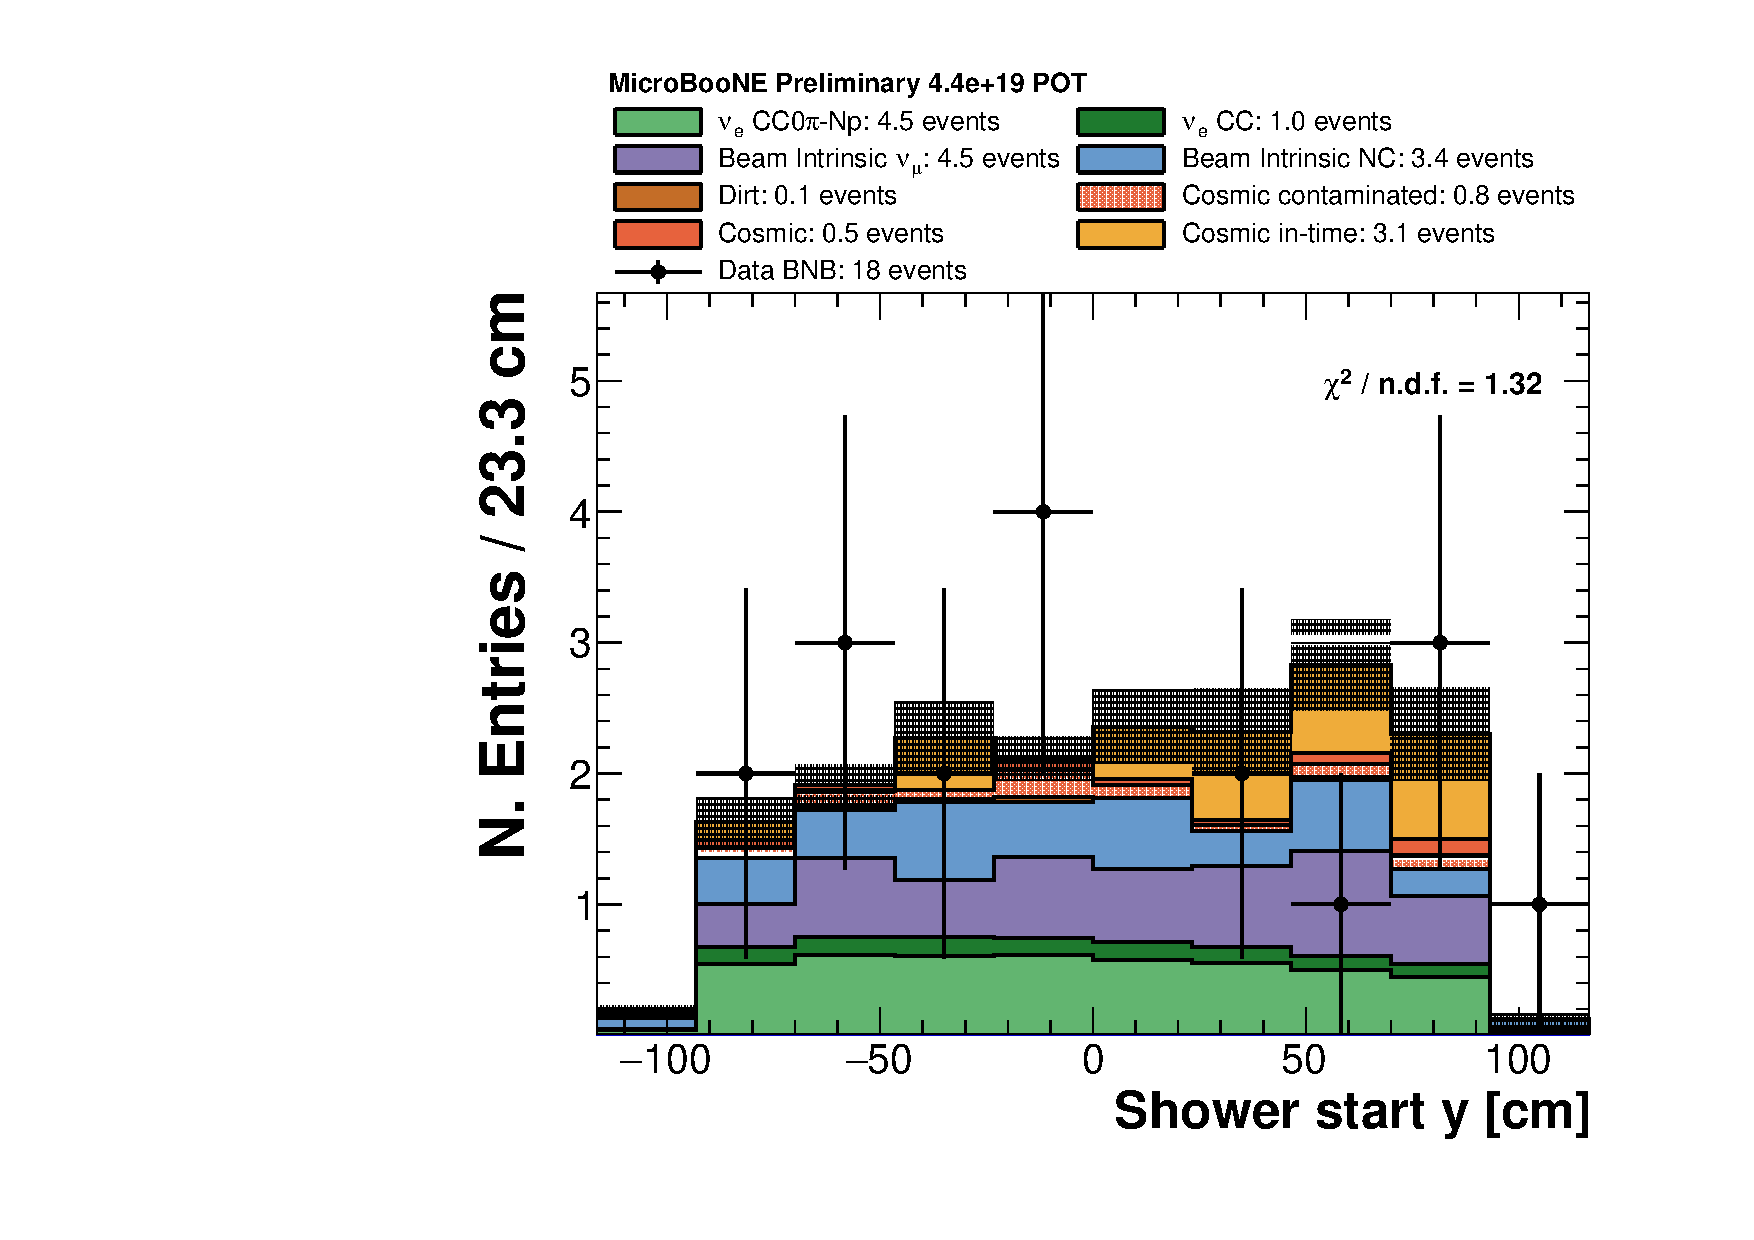
\includegraphics[width=\linewidth]{figures/h_shower_start_y.pdf}
    \caption{$y$ coordinate.} 
  \end{subfigure}
  \begin{subfigure}{0.3\textwidth}
    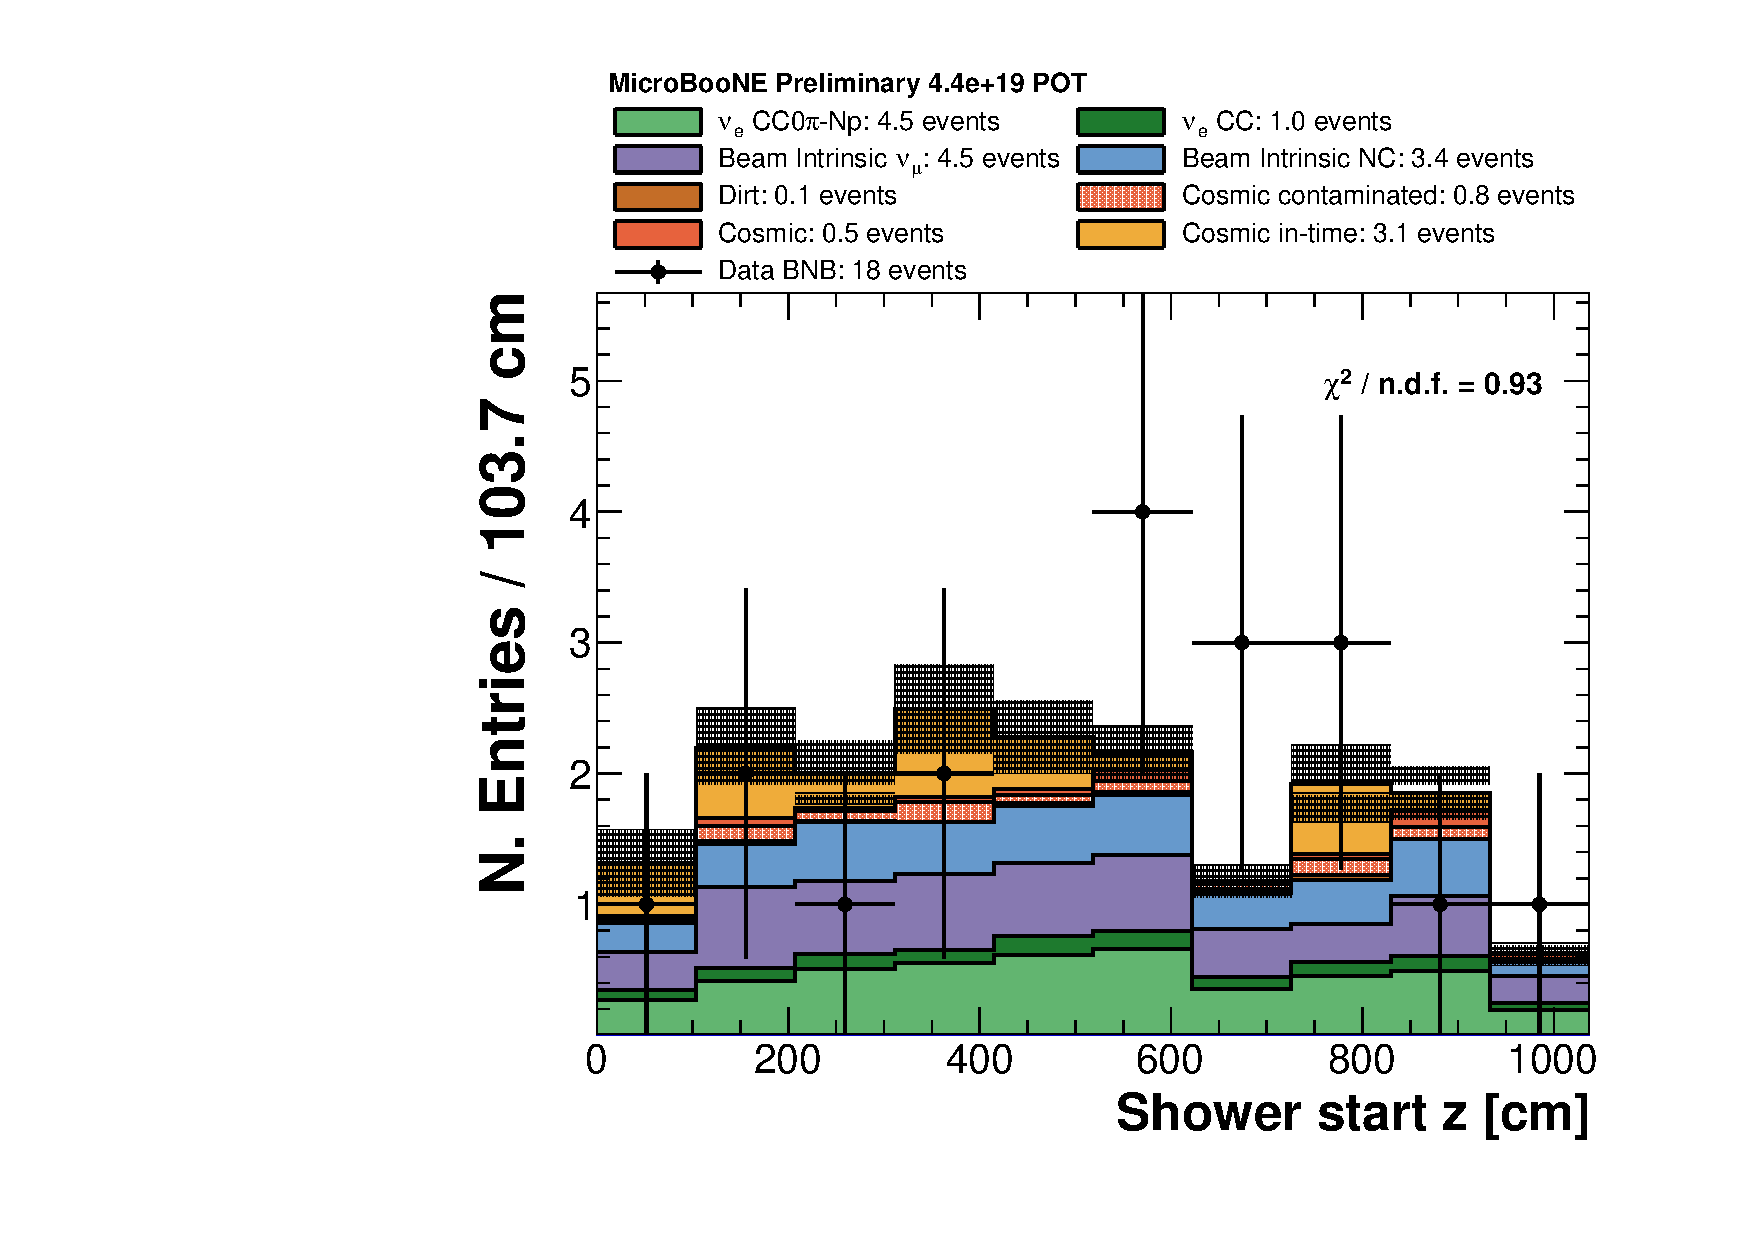
\includegraphics[width=\linewidth]{figures/h_shower_start_z.pdf}
    \caption{$z$ coordinate.} 
  \end{subfigure}
  \caption{Distribution of the starting point of the most energetic reconstructed shower in each event in the $x$, $y$, and $z$ coordinates.}\label{fig:showerxyz}
\end{figure}

Figure \ref{fig:showerangles} shows the distributions of the inclination $\theta$ and azimuth $\phi$ angles of the most energetic reconstructed shower in each event. As expected, the selected events are mainly forward-going ($\theta < 90^{\circ}$) and evenly distributed on the azimuth angle.

\begin{figure}[htbp]
\centering
  \begin{subfigure}{0.45\textwidth}
    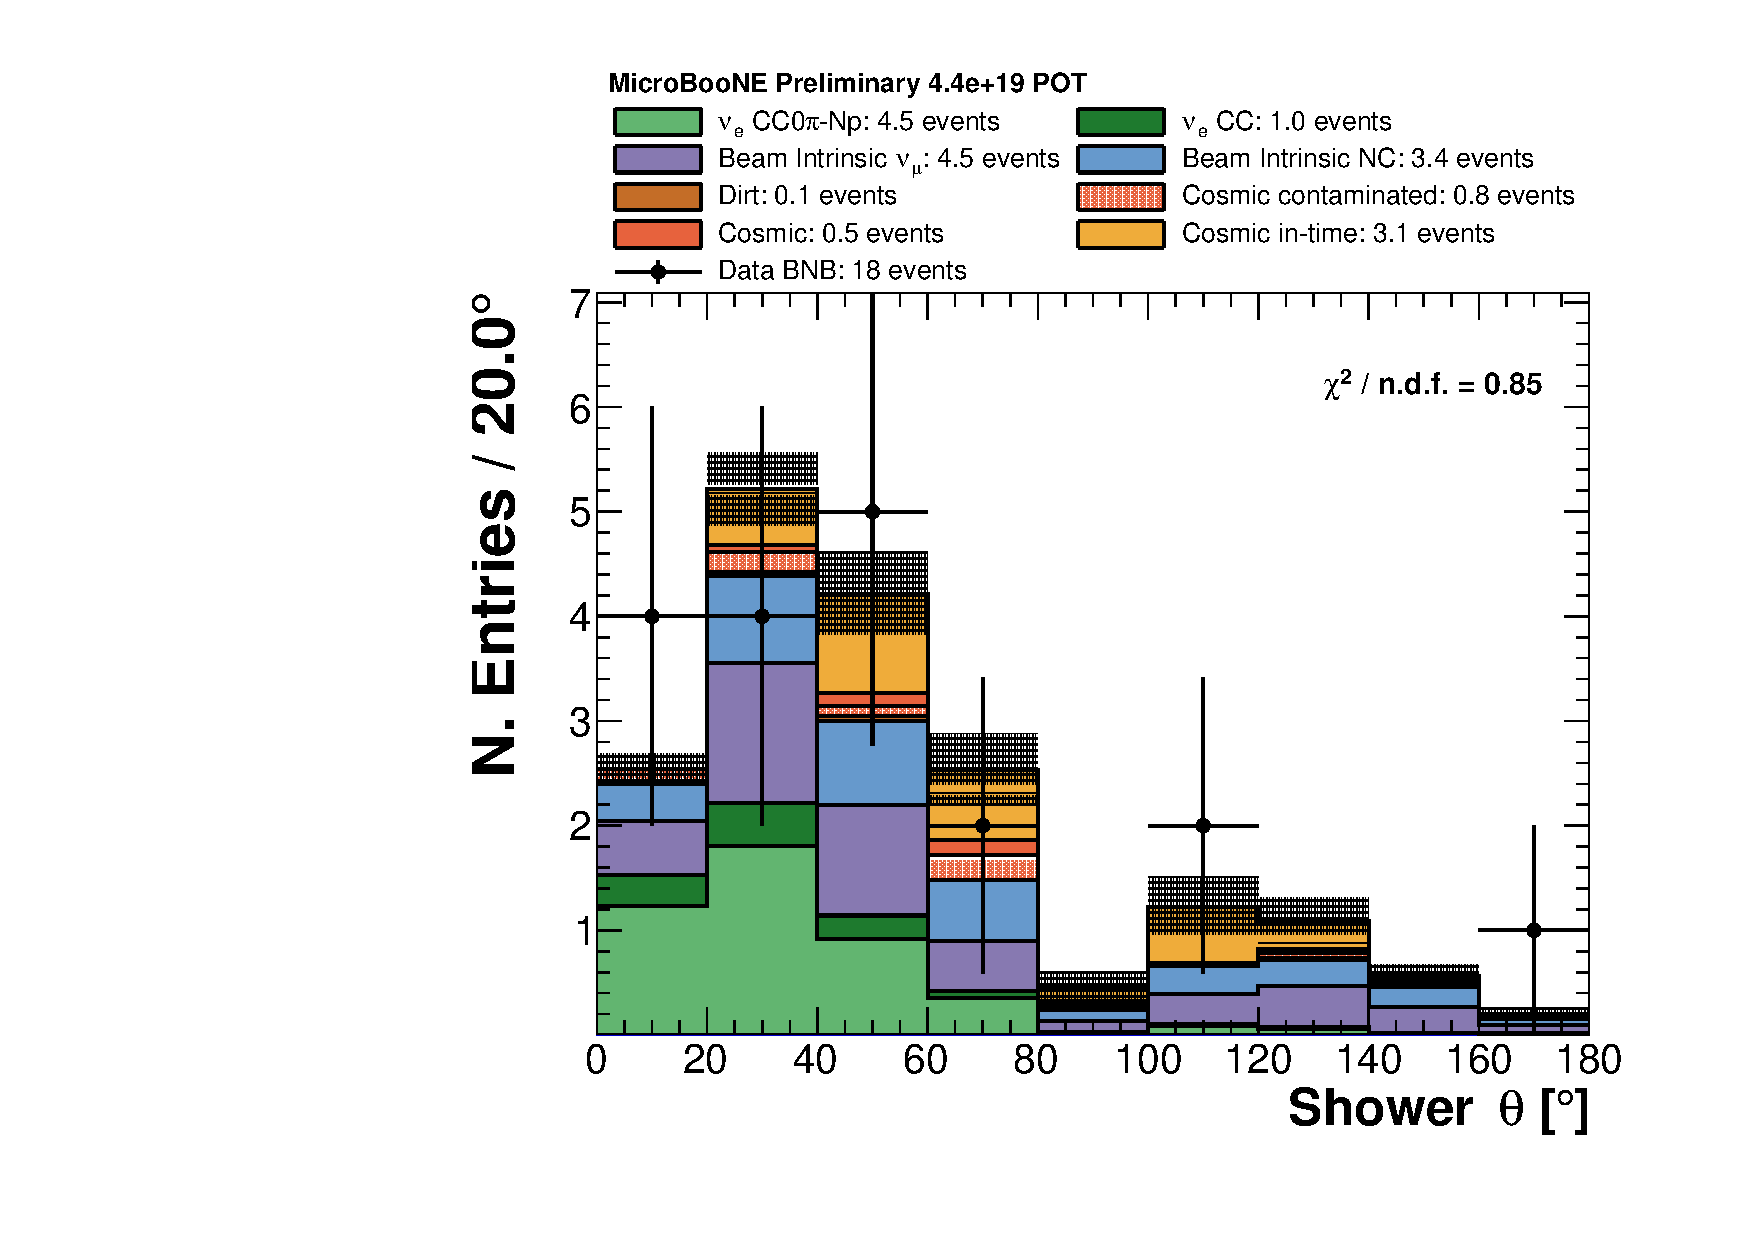
\includegraphics[width=\linewidth]{figures/h_shower_theta_after.pdf}
    \caption{Inclination $\theta$.} 
  \end{subfigure}
    \begin{subfigure}{0.45\textwidth}
    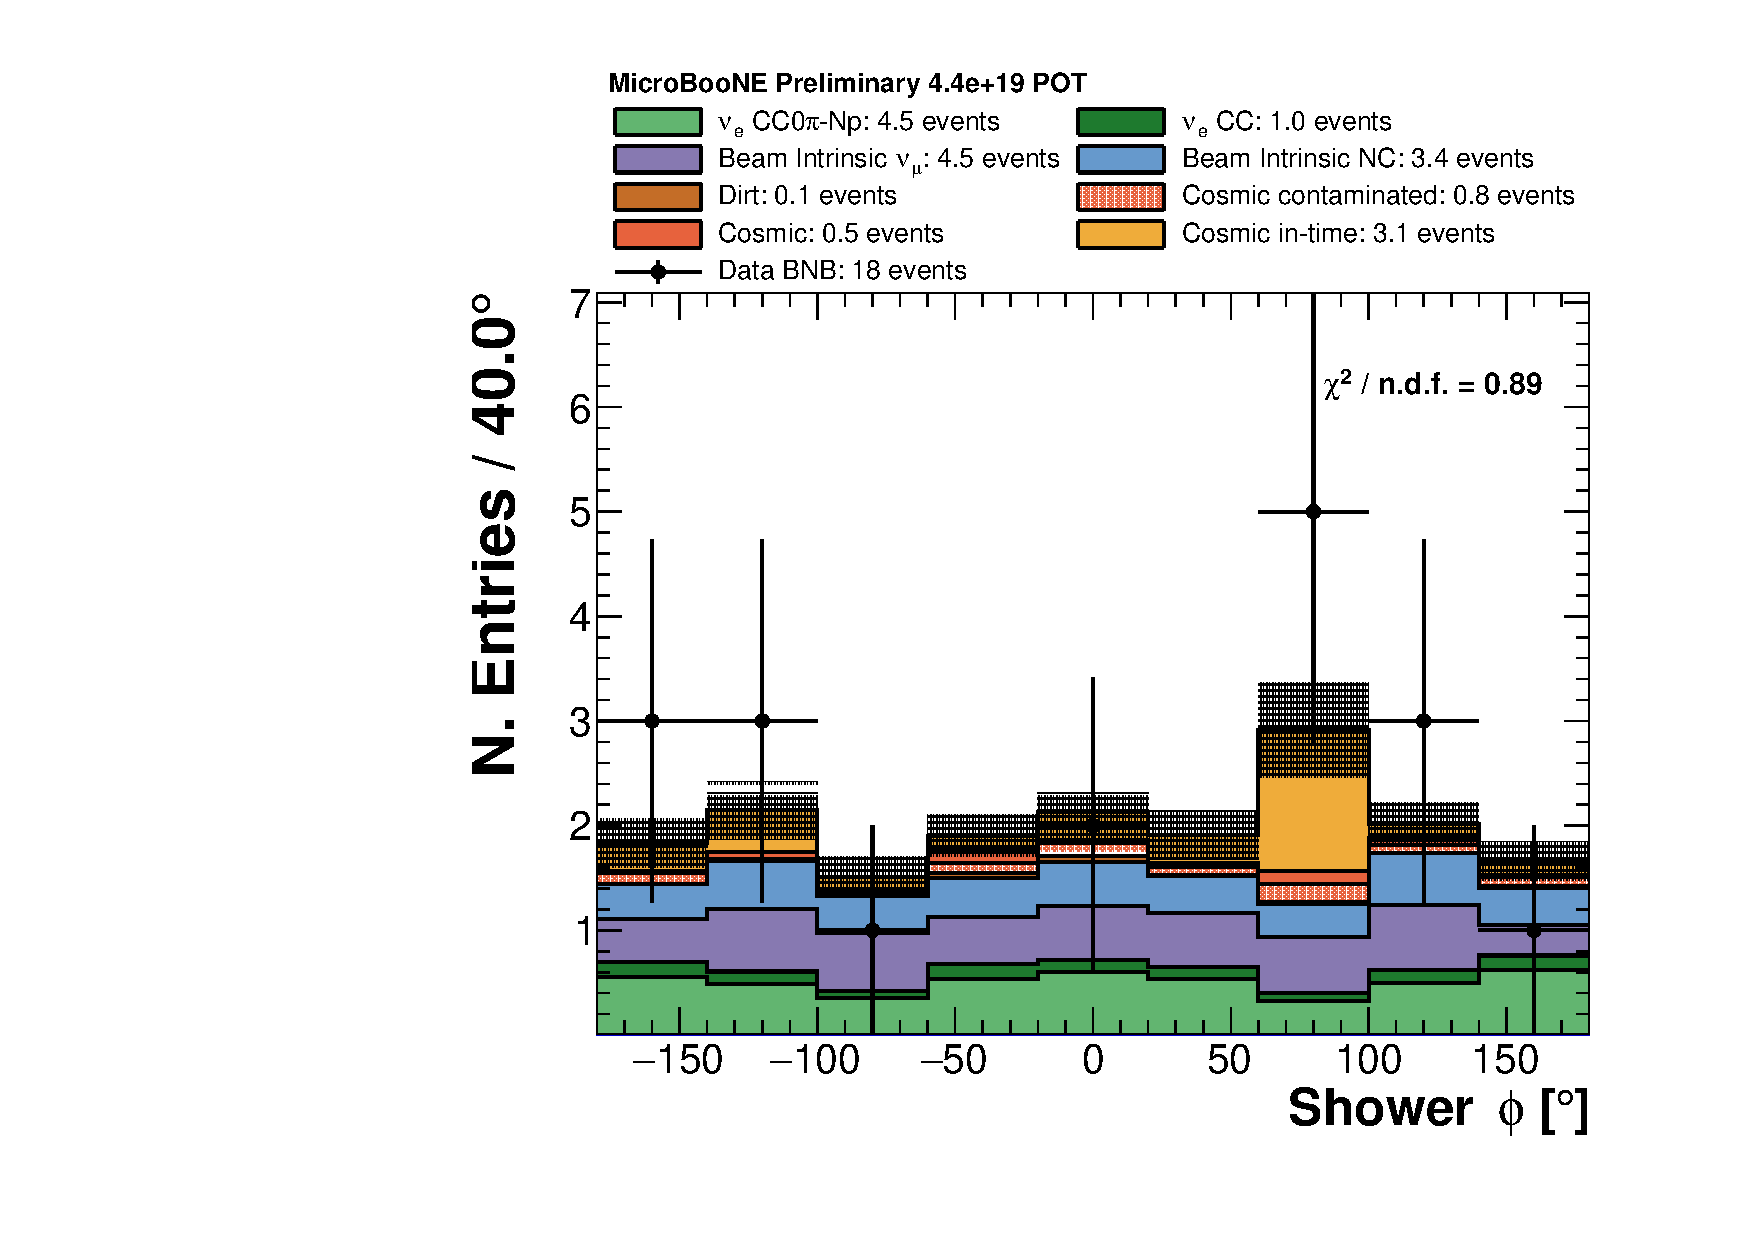
\includegraphics[width=\linewidth]{figures/h_shower_phi_after.pdf}
    \caption{Azimuth $\phi$.} 
  \end{subfigure}
  \caption{Distribution of the inclination $\theta$ and azimuth $\phi$ angles of the most energetic reconstructed shower in each event.}\label{fig:showerangles}
\end{figure}


\subsection{Efficiency and purity}
It is now possible to calculate the efficiency and the purity of our $\nu_{e}$ CC0$\pi$-Np selection after the background-rejection cuts, as defined in Section \ref{sec:eff}. The background-rejection cuts were aimed to improve the significance of the $\nu_{e}$ CC0$\pi$-Np events in our sample. Thus, the efficiency decreases, from 41.1\% to 14.3\%, since the cuts will eventually remove also some signal events, but the purity increases by a factor of $\sim50$, from 0.5\% to 24.0\%. 
Table \ref{tab:cutflow} shows the $\nu_{e}$ CC0$\pi$-Np efficiency and purity for each cut, applied in sequentially.

\begin{table}[htbp]
   \centering
   \begin{tabular}{llrrrrrrrr}
     \toprule
     Step & \phantom{a} & Signal & \phantom{a} & Background & \phantom{a} & Efficiency & \phantom{a} & Purity\\
     \midrule

     Generation           & & 34.8     & & 14.3   & & 4.9   & & 14.3\%\\
     Optical and topology & & 35.7     & & 13.2   & & 1.6   & & 4.5\%\\
     Quality pre-cuts     & & 11337.4  & & 918.3  & & 4.8   & & 0.04\%\\
     Shower $dE/dx$       & & 3633.9   & & 342.2  & & 3.6   & & 0.1\%\\
     Shower energy        & & 2609.5   & & 37.1   & & 0.2   & & 0.008\%\\
     Proton track BDT     & & 135377.2 & & 1151.6 & & 3.5   & & 0.003\%\\
     Track distance       & & -        & & 260.7  & & 1.1   & & 0.4\%\\
     Shower distance      & & -        & & 233.3  & & 0.7   & & 0.3\%\\
     Track-shower angle   & & -        & & 233.3  & & 0.7   & & 0.3\%\\
	 Shower opening angle & & -        & & 233.3  & & 0.7   & & 0.3\%\\
     Track length         & & -        & & 233.3  & & 0.7   & & 0.3\%\\
     \bottomrule
   \end{tabular}
   \caption{Efficiency and purity after each cuts applied on the generated samples of Monte Carlo events.}\label{tab:cutflow}
\end{table}

Figure \ref{fig:effafter} shows the efficiency as a function of the true neutrino energy and the purity as a function of the reconstructed energy, before and after the background rejection cuts. 

\begin{figure}
  \begin{subfigure}{0.48\textwidth}
    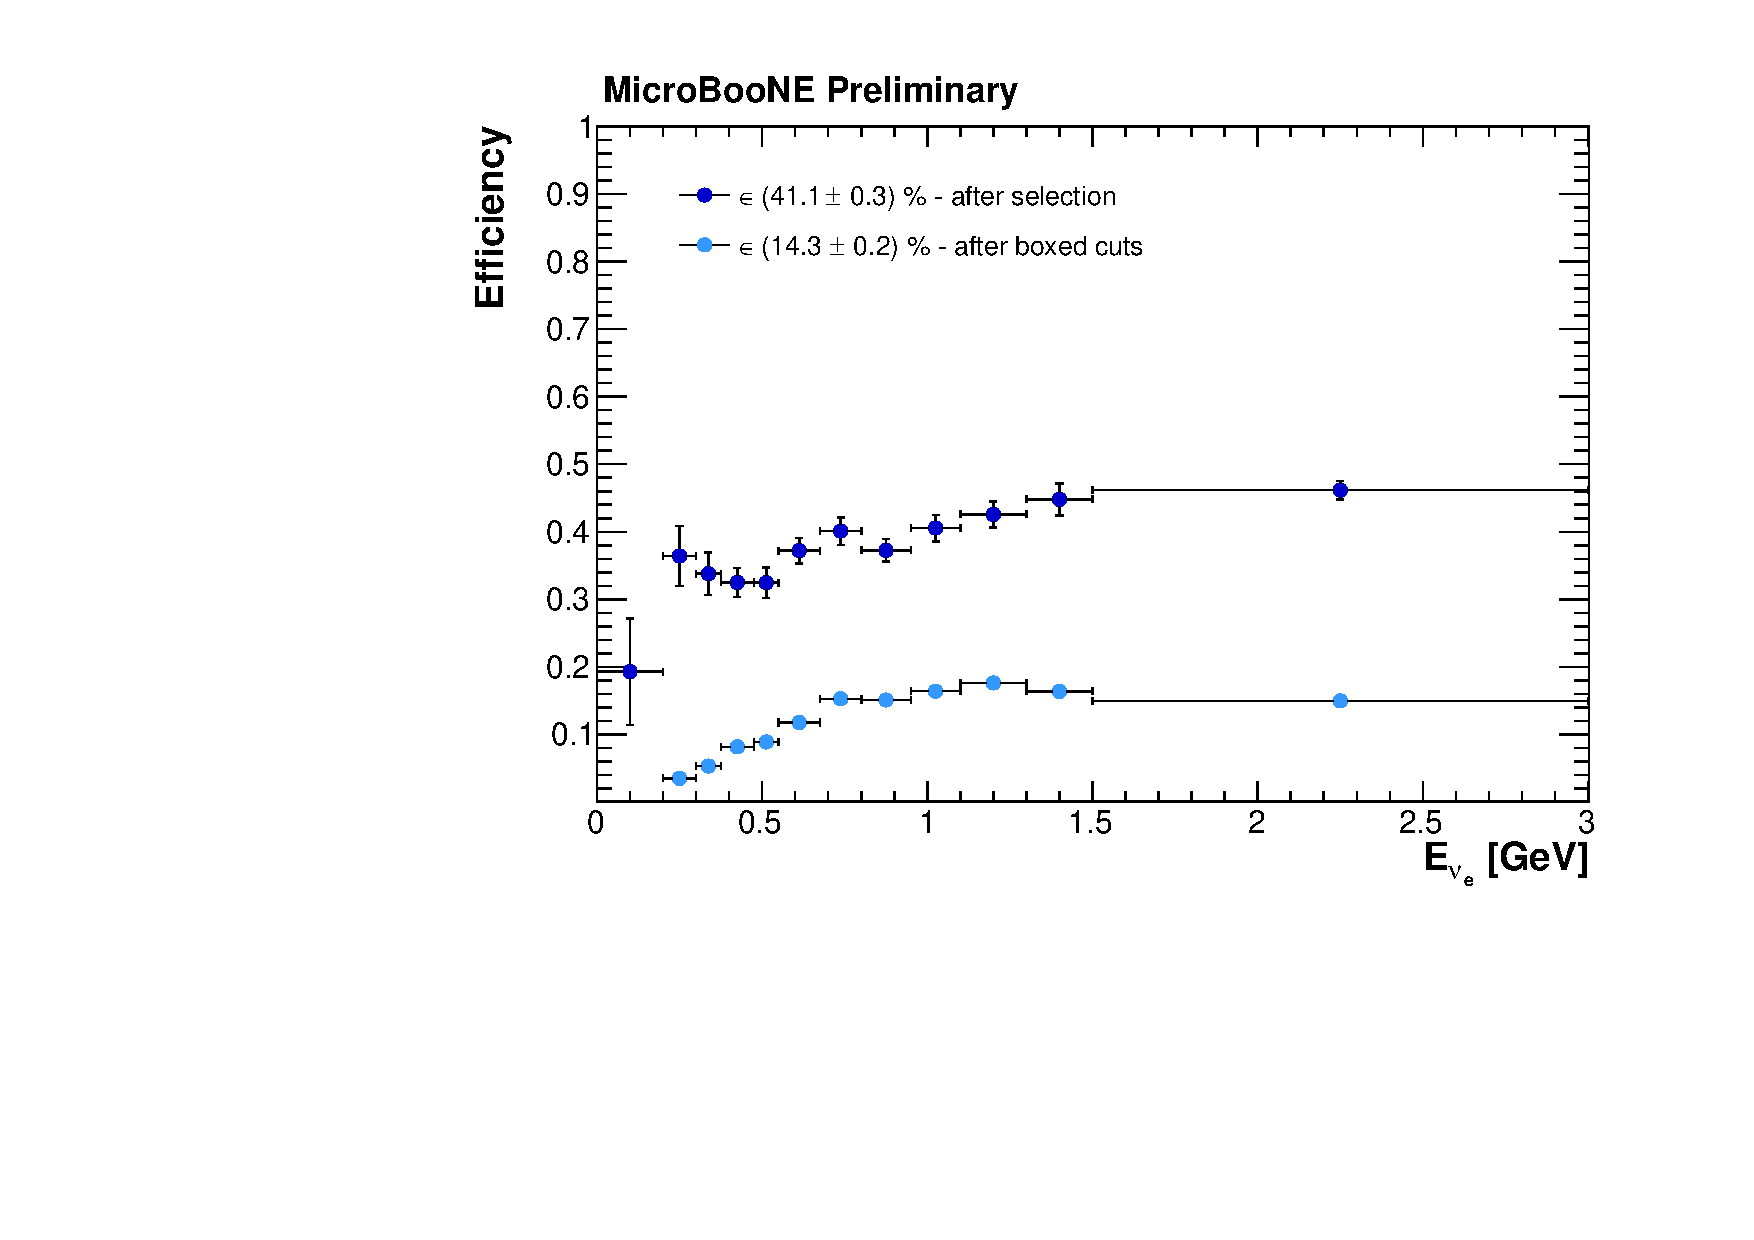
\includegraphics[width=\linewidth]{figures/eff_after.pdf}
    \caption{Efficiency} 
  \end{subfigure}
    \begin{subfigure}{0.48\textwidth}
    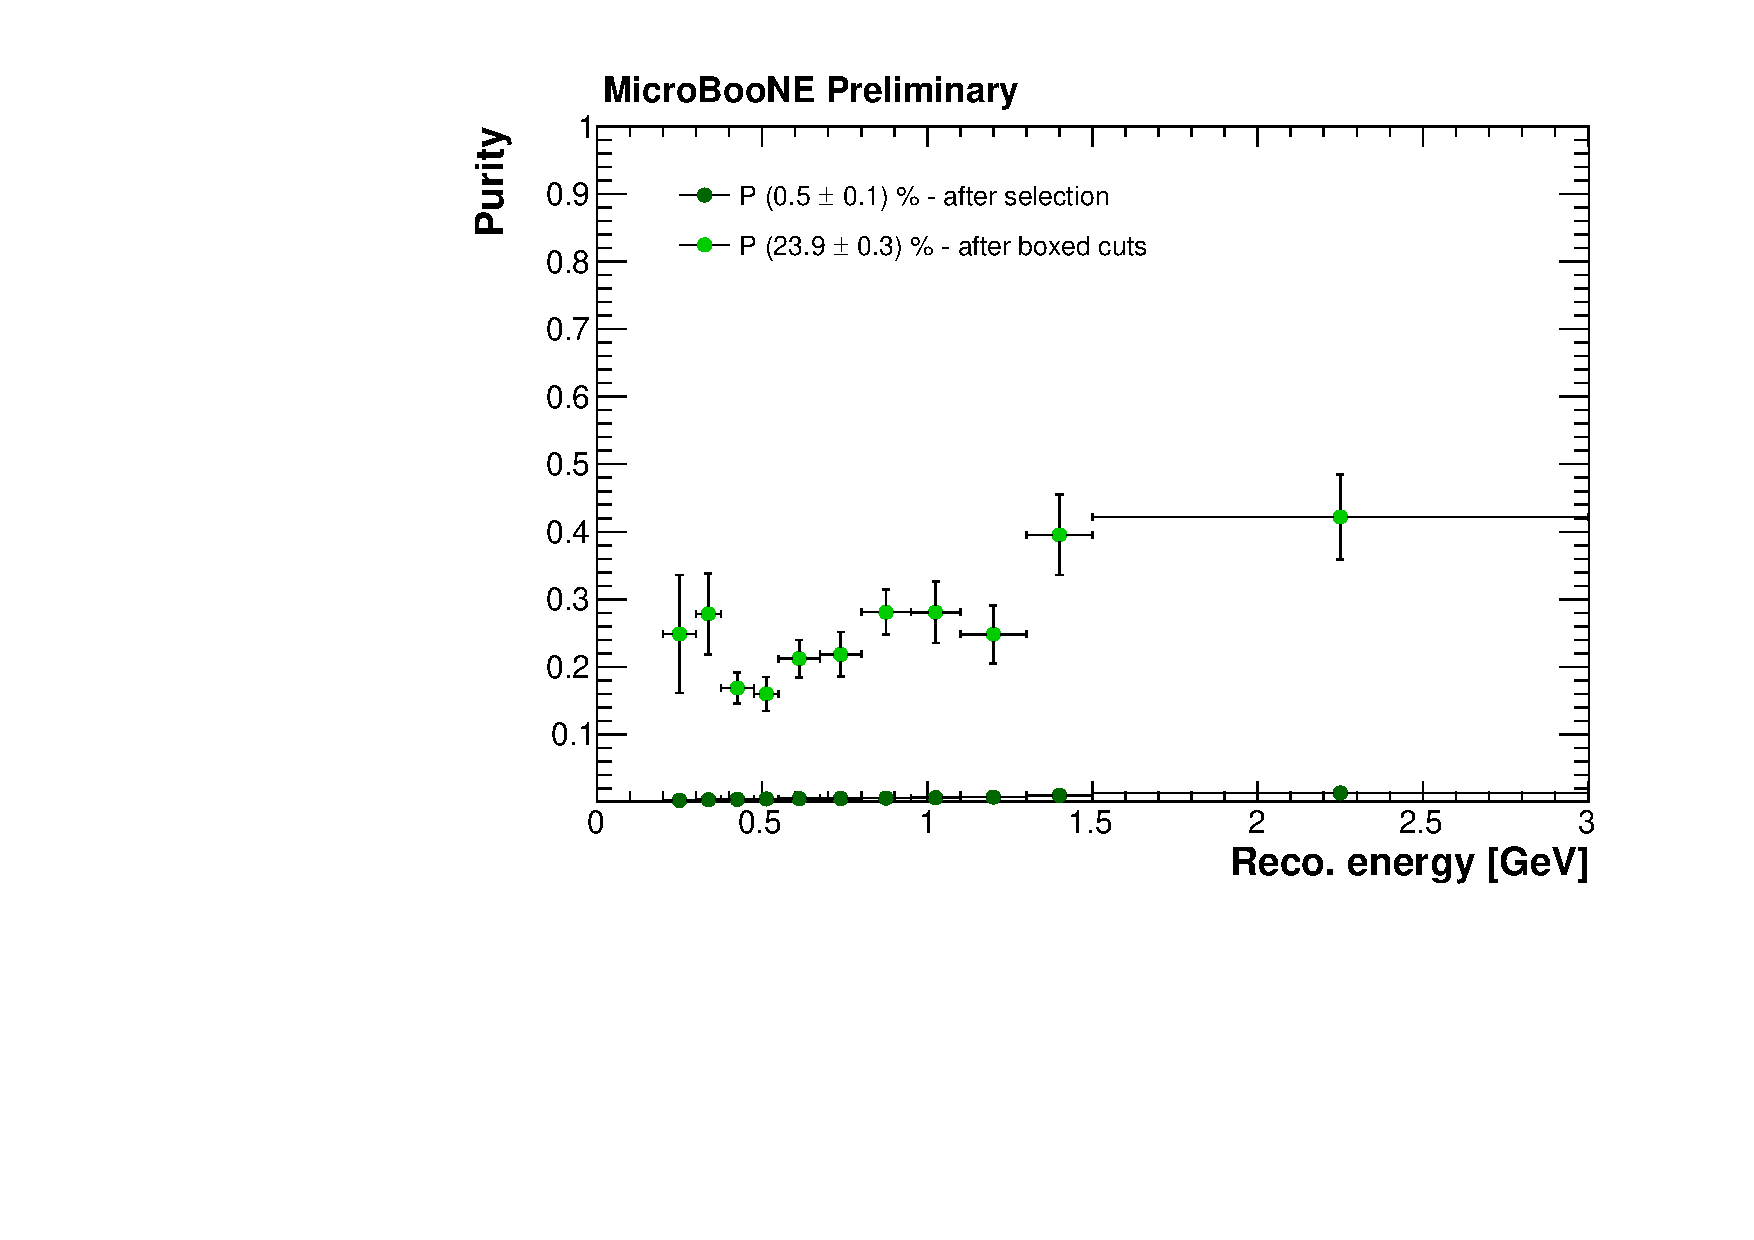
\includegraphics[width=\linewidth]{figures/purity_after.pdf}
    \caption{Purity} 
  \end{subfigure}
  \caption{Left: $\nu_{e}$ CC$0\pi$-Np reconstruction efficiency as a function of the true $\nu_{e}$ energy before and after the background-rejection cuts. Right: $\nu_{e}$ CC$0\pi$-Np purity as a function of the reconstructed energy before and after the background-rejection cuts.}
  \label{fig:effafter}
\end{figure}

Table \ref{tab:effafter} shows the efficiency and the number of events selected for each event category before and after the background-rejection cuts. In particular, we are able to reject the 99.5\% of the neutrino background and the 
99.996\% of the cosmogenic background, while retaining a 14.3\% $\nu_{e}$ CC0$\pi$-Np efficiency.

\begin{table}[htbp]
   \centering
   \begin{tabular}{llrrrrrrrr}
     \toprule
     Category & \phantom{a} & Generated & \phantom{a} & Selected & \phantom{a} & After cuts & \phantom{a} & Efficiency\\
     \midrule

     $\nu_{e}$ CC0$\pi$-Np       & & 34.8     & & 14.3   & & 4.9   & & 14.3\%\\
     $\nu_{e}$ CC                & & 35.7     & & 13.2   & & 1.6   & & 4.5\%\\
     Beam intrinsic $\nu_{\mu}$  & & 11337.4  & & 918.3  & & 4.8   & & 0.04\%\\
     Beam intrinsic NC           & & 3633.9   & & 342.2  & & 3.6   & & 0.1\%\\
     Outside fid. vol.           & & 2609.5   & & 37.1   & & 0.2   & & 0.008\%\\
     Cosmic in-time              & & 135377.2 & & 1151.6 & & 3.5   & & 0.003\%\\
     Cosmic contaminated         & & -        & & 260.7  & & 1.1   & & 0.4\%\\
     Cosmic                      & & -        & & 233.3  & & 0.7   & & 0.3\%\\

     \bottomrule
   \end{tabular}
   \caption{Summary of the selection algorithm results, showing the contribution of each event category, for a MicroBooNE exposure of \num{4.84e19} POT.}\label{tab:effafter}
\end{table}

\subsubsection{Selection with increased purity}
It is possible to apply stricter cuts in order to increase the purity of our selected sample. However, stricter cuts will correspond to a lower efficiency and also to a lower total number of selected data events, making the validation of this new set of cuts more difficult.
Figure \ref{fig:hardcuts} shows the reconstructed energy spectrum of the selected events with:
\begin{itemize}
\item Distance of the most proton-like track < 2.5~cm (instead of 3~cm)
\item 1.6~MeV/cm < $dE/dx$ of the most energetic shower < 2.6~MeV/cm (was 1.2~MeV/cm < $dE/dx$ < 3.2~MeV/cm)
\item BDT score of the most proton-like tracks > 0 (was > -0.12).
\end{itemize}
These stricter cuts allow to achieve a purity larger than 50\% (51.5\%), decreasing however the efficiency from 14.3\% to 8.9\%. In particular, the \emph{cosmic in-time} background component is completely removed from the selected sample.
The number of events have been scaled in this case to the predicted exposure of the MicroBooNE detector of \num{6.6e20} POT. 

\begin{figure}[htbp]
\centering
  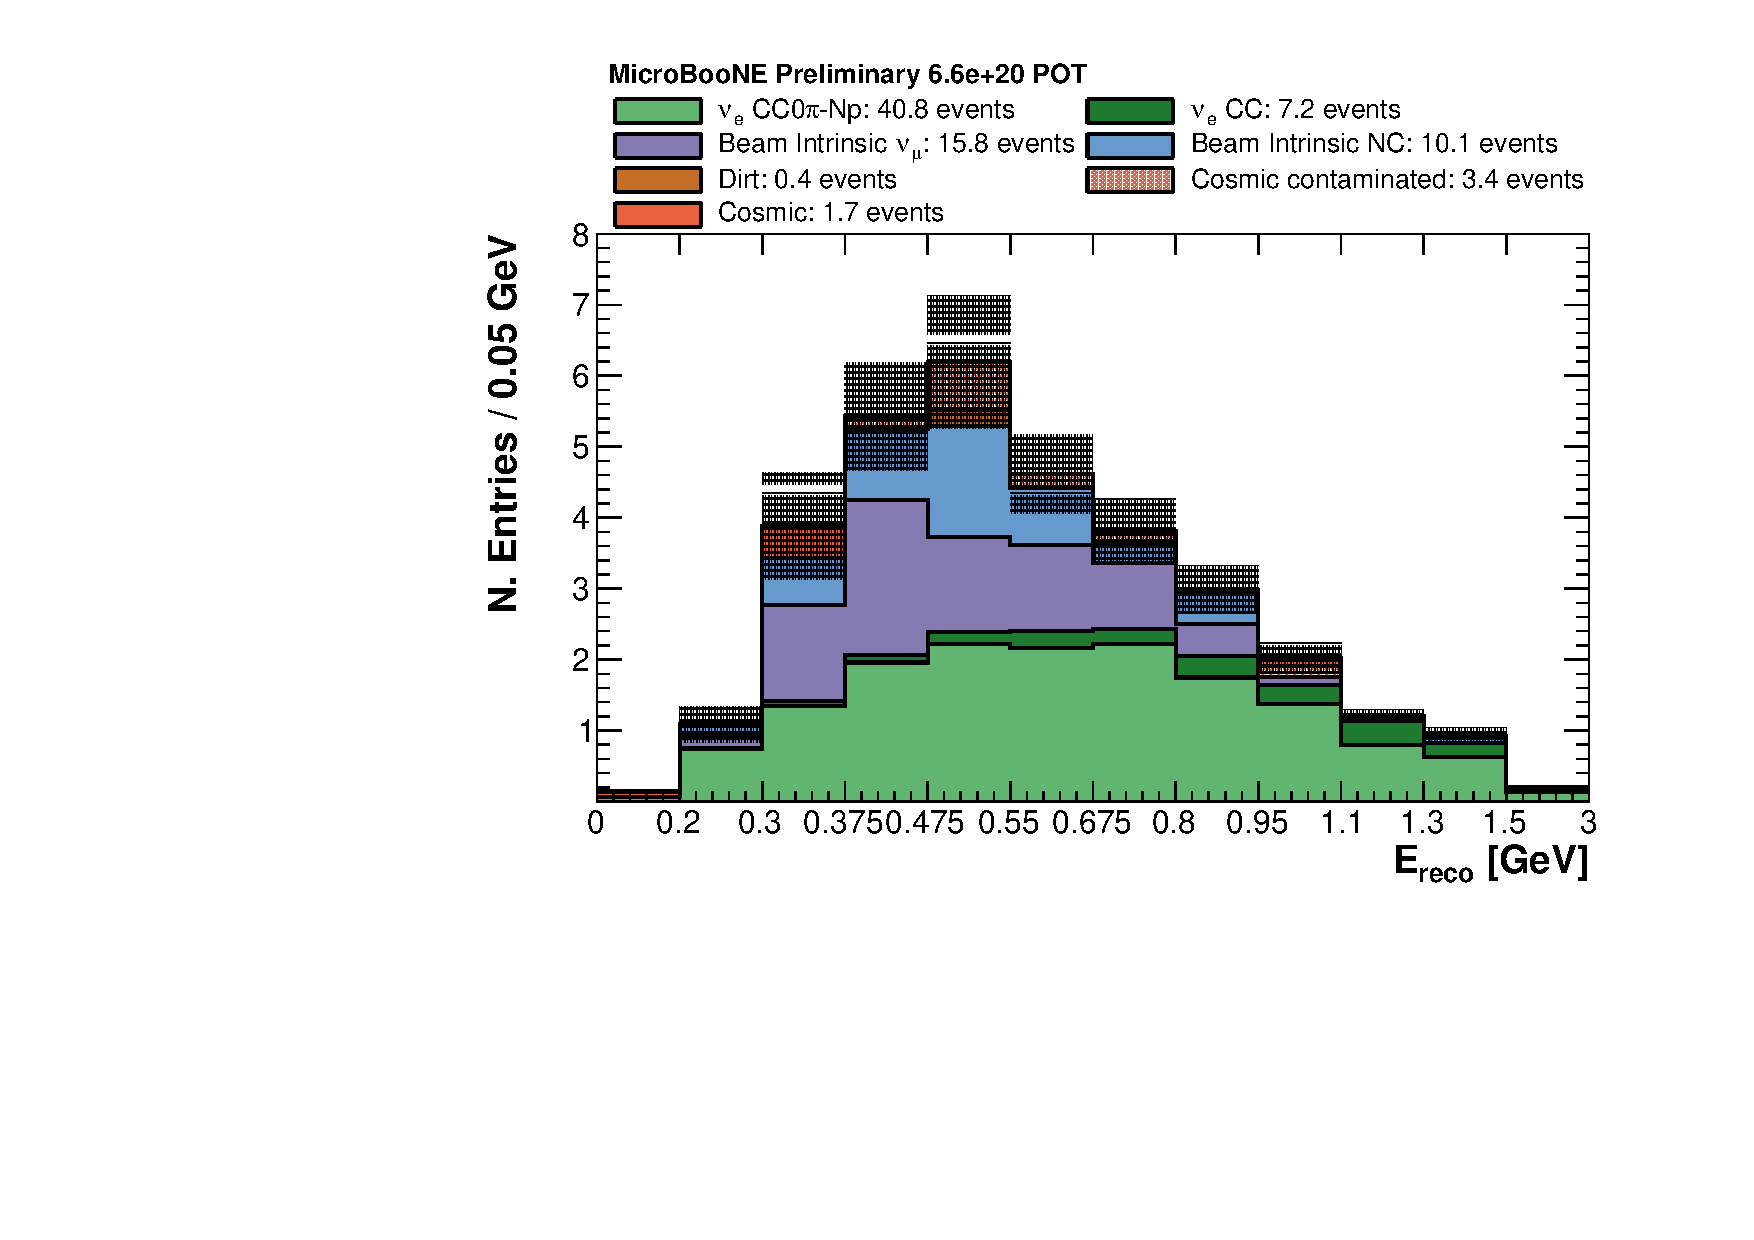
\includegraphics[width=0.65\linewidth]{figures/hardcuts.pdf}
  \caption{Reconstructed energy spectrum of the selected events after stricter background-rejecting cuts. Numbers of events have been scaled to the predicted exposure of the MicroBooNE detector of \num{6.6e20} POT. }
  \label{fig:hardcuts}
\end{figure}